\documentclass[11pt]{article}
\usepackage[margin=1.05in]{geometry}
\usepackage{amsmath,amssymb,bm}
\usepackage{booktabs}
\usepackage{siunitx}
\usepackage{graphicx}
\usepackage{tikz}
\usetikzlibrary{arrows.meta,positioning}
\usepackage{listings}
\usepackage{xcolor}
\usepackage[colorlinks=true,linkcolor=blue,citecolor=blue,urlcolor=blue]{hyperref}

\newcommand{\ud}{\,\mathrm{d}}
\newcommand{\vect}[1]{\bm{#1}}
\newcommand{\file}[1]{\texttt{#1}}

\lstset{basicstyle=\ttfamily\footnotesize, frame=single, framesep=4pt,
        backgroundcolor=\color{gray!6}, columns=fullflexible,
        breaklines=true, showstringspaces=false}

\tikzset{
  stage/.style={draw, rounded corners=2pt, align=center, font=\small,
                minimum height=8mm, inner xsep=5pt, fill=green!6},
  opt/.style={stage, fill=gray!8, densely dashed},
  data/.style={draw, align=center, font=\scriptsize\ttfamily, fill=yellow!10,
               minimum height=7mm, inner xsep=4pt},
  fl/.style={-{Stealth[length=2mm]}, thick},
}

\title{GTO $\to$ ELFO: \\
Problem, Formulation, Discretization, and How to Run It}
\author{Michael Casey}
\date{July 26, 2026}

\begin{document}
\maketitle

\begin{abstract}
A working guide to the direct (collocation) solution of the minimum-fuel
low-thrust transfer from GTO to an Elliptical Lunar Frozen Orbit (ELFO) in the
Earth--Moon CR3BP. The transfer problem, the optimal control problem, the
discretization --- which differs from its tulip sibling in one substantive way,
a \emph{free} final time carried as a slack state --- the pipeline, how to run
it, and what is and is not established. Written 2026-07-26; this campaign had
no technical document before it.
\end{abstract}

\tableofcontents

%=======================================================================
\section{The transfer problem}
%=======================================================================

The spacecraft is the same as the tulip campaign's --- \SI{15}{\kilo\gram},
\SI{25}{\milli\newton}, $I_{sp}=\SI{2100}{\second}$ --- and so is the dynamical
model: the circular restricted three-body problem in the rotating Earth--Moon
frame, non-dimensionalized on $l^\ast$ and $t^\ast$. What changes is the
target. Instead of a south-pole tulip orbit, the spacecraft must arrive on an
\emph{elliptical lunar frozen orbit}: a lunar orbit whose eccentricity and
argument of periapsis are stationary under the dominant perturbations, which is
what makes it attractive for sustained south-pole coverage.

The insertion state is produced by \file{gto\_elfo\_endpoints.m} through
\file{insertion\_states('elfo', criterion)}, with three criteria available ---
\texttt{'nearest'} (the default, the point on the ELFO nearest the tulip
campaign's insertion, so the two campaigns are comparable),
\texttt{'apolune'}, and \texttt{'perilune'}. As in the tulip campaign, both
endpoints come from that single function, so every ELFO pipeline starts and
ends at identical numbers.

The campaign's time anchor is its own:
\begin{center}
\begin{tabular}{lll}
\toprule
quantity & value & source \\
\midrule
$t_{f,\min}^{\text{ELFO}}$ & $6.0961535$ ND $=\SI{27.02}{\day}$
   & certified direct all-burn (Route B) \\
\bottomrule
\end{tabular}
\end{center}

\noindent This matters and has bitten before: ELFO factors are
$t_f/t_{f,\min}^{\text{ELFO}}$, \emph{not} $t_f/t_{f,\min}^{\text{tulip}}$.
Before 2026-07-21 ELFO factors were mislabelled against the tulip anchor. The
physical $t_f$ values were correct; the labels were not.

%=======================================================================
\section{The optimal control problem}
%=======================================================================

The continuous problem is the tulip campaign's with a different terminal
manifold. With $\vect{r},\vect{v}$ in the rotating frame, mass $m$, throttle
$s\in[0,1]$ and unit direction $\vect{\alpha}$:
\begin{align}
\dot{\vect{r}} &= \vect{v}, \\
\dot{\vect{v}} &= -2\,\vect{\omega}\times\vect{v}
   - \vect{\omega}\times(\vect{\omega}\times\vect{r})
   -\frac{(1-\mu^\ast)}{r_1^3}\vect{r}_1
   -\frac{\mu^\ast}{r_2^3}\vect{r}_2
   +\frac{T_{\max}}{m}\,s\,\vect{\alpha}, \\
\dot{m} &= -\frac{T_{\max}}{c}\,s ,
\end{align}
subject to $\|\vect{\alpha}\|=1$, fixed initial state on GTO, fixed terminal
state on the ELFO, $m(0)$ given, $m(t_f)$ free.

The objective and its treatment are identical to the tulip campaign's: minimum
fuel is linear in $s$, hence bang--bang, hence solved through the
Bertrand--\'Epenoy homotopy
\begin{equation}
J(\varepsilon)=\int_0^{t_f}\big[s-\varepsilon\,s(1-s)\big]\ud t,
\qquad \varepsilon:1\to0 ,
\label{eq:hom}
\end{equation}
with $\varepsilon=1$ the smooth minimum-energy root and $\varepsilon=0$ pure
minimum fuel.

%=======================================================================
\section{Discretization: the free-time formulation}
%=======================================================================

This is where ELFO genuinely departs from its sibling, and it is the reason
this campaign has its own solvers (\file{casadi\_energy\_freetf.m},
\file{casadi\_mintime\_freetf.m}) rather than reusing the tulip engine.

\subsection{The problem with a fixed pseudo-time horizon}

Both campaigns use the Sundman transformation $\ud t/\ud\tau=\kappa$ to
concentrate mesh where the dynamics are stiff. The tulip campaign holds the
final pseudo-time $\tau_f$ \emph{fixed} and enforces the physical horizon as a
terminal condition $t(\tau_f)=t_f$. That keeps the KKT matrix banded, at the
cost that the trajectory's winding number cannot grow --- which is exactly what
blocks its thrust ladder.

Making $\tau_f$ a free scalar decision variable removes that restriction but
reintroduces the problem it was avoiding: a scalar coupled to every node
produces a dense column in the KKT matrix, and at several thousand nodes the
sparse factorization runs out of memory.

\subsection{Betts' slack-state trick}

The resolution is to carry the free time as a \emph{state} rather than a
scalar. Introduce a ninth state $c$ (\texttt{cScale}) with
\begin{equation}
\frac{\ud t}{\ud\tau} \;=\; c\,\kappa ,
\qquad
\frac{\ud c}{\ud\tau} \;=\; 0 .
\end{equation}
The second equation, discretized, is a set of \emph{local} continuity
constraints tying $c$ across adjacent nodes. It is therefore one number
functionally, but structurally it is banded like every other state --- no dense
column, no factorization blow-up. The state becomes
\[
\vect{x} \;=\; \big(\vect{r},\ \vect{v},\ m,\ t,\ c\big)\in\mathbb{R}^9 ,
\qquad
\vect{u} \;=\; \big(\vect{\alpha},\ s\big)\in\mathbb{R}^4 .
\]
The objective in \eqref{eq:hom} is integrated against the physical-time measure
$\ud t=c\,\kappa\ud\tau$, so the cost remains a genuine time integral.

Two regimes then fall out of one solver:
\begin{itemize}
\item \textbf{Pinned $t_f$}: add $t(\tau_f)=t_{\text{target}}$ and let $c$
float to satisfy it. This is the normal mode --- the horizon is what the user
asked for, and $c$ absorbs the pseudo-time/physical-time mismatch.
\item \textbf{Genuinely free $t_f$}: leave the terminal time constraint off.
Used for the minimum-time anchor, where $t_f$ \emph{is} the objective.
\end{itemize}

\subsection{The nonlinear program}

Trapezoidal collocation on a uniform $\tau$ grid, defects
\begin{equation}
\vect{x}_{k+1}-\vect{x}_k-\frac{h}{2}\big[\vect{f}_{k+1}+\vect{f}_k\big]=\vect{0},
\end{equation}
with $\|\vect{\alpha}_k\|=1$ and $0\le s_k\le1$ nodewise, assembled in CasADi
and solved by IPOPT with exact sparse AD derivatives.

%=======================================================================
\section{The pipeline}
%=======================================================================

\begin{figure}[htbp]
\centering
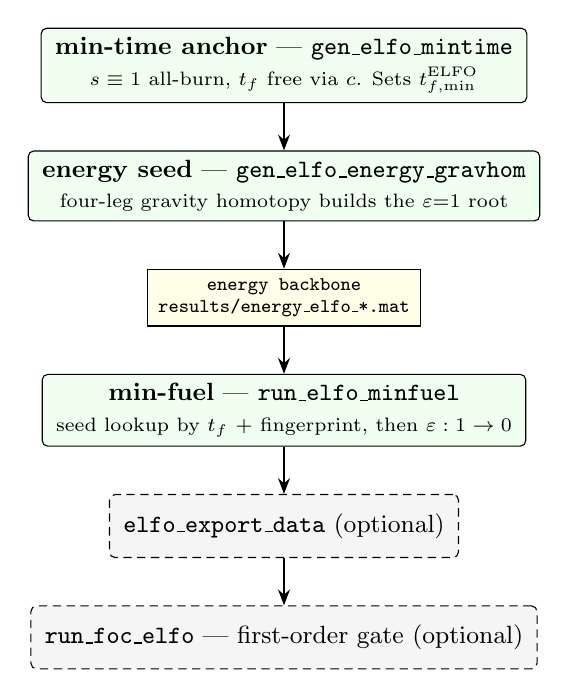
\begin{tikzpicture}[node distance=6mm]
  \node[stage] (mt) {\textbf{min-time anchor} --- \file{gen\_elfo\_mintime}\\
        \scriptsize $s\equiv1$ all-burn, $t_f$ free via $c$. Sets $t_{f,\min}^{\text{ELFO}}$};
  \node[stage, below=of mt] (gh) {\textbf{energy seed} --- \file{gen\_elfo\_energy\_gravhom}\\
        \scriptsize four-leg gravity homotopy builds the $\varepsilon{=}1$ root};
  \node[data, below=of gh] (bb) {energy backbone\\ \file{results/energy\_elfo\_*.mat}};
  \node[stage, below=of bb] (mf) {\textbf{min-fuel} --- \file{run\_elfo\_minfuel}\\
        \scriptsize seed lookup by $t_f$ + fingerprint, then $\varepsilon:1\to0$};
  \node[opt, below=of mf] (ex) {\file{elfo\_export\_data} (optional)};
  \node[opt, below=of ex] (fc) {\file{run\_foc\_elfo} --- first-order gate (optional)};
  \draw[fl] (mt) -- (gh); \draw[fl] (gh) -- (bb);
  \draw[fl] (bb) -- (mf); \draw[fl] (mf) -- (ex); \draw[fl] (ex) -- (fc);
\end{tikzpicture}
\caption{The ELFO pipeline. Unlike the tulip campaign there is no single
six-stage front door; the stages are separate drivers, chained by banked
artifacts and orchestrated for sweeps by shell scripts.}
\label{fig:elfopipe}
\end{figure}

\paragraph{The gravity homotopy.} The ELFO energy seed is harder to obtain
than the tulip's, because the terminal manifold sits deep in the Moon's
potential well. \file{gen\_elfo\_energy\_gravhom} walks a four-leg homotopy
that brings lunar gravity up gradually, converting a converged solution at
reduced lunar influence into one at full strength.

\paragraph{Seed selection is fingerprinted.} \file{elfo\_find\_energy\_seed}
picks a banked seed by $t_f$ \emph{and} by a physics fingerprint (thrust, mass,
$I_{sp}$, endpoints). A nominal \SI{25}{\milli\newton} seed will not be served
to a \SI{20}{\milli\newton} request; the filter refuses rather than silently
warm-starting from the wrong physics.

%=======================================================================
\section{How to run it}
%=======================================================================

\begin{lstlisting}[language=Matlab]
cd orbit_transfer/GTO_ELFO/direct/elfo
setup_paths

gen_elfo_mintime                 % the Route-B min-time anchor
gen_elfo_energy_gravhom          % build an energy backbone (gravity homotopy)
run_elfo_minfuel                 % energy -> fuel at a chosen t_f
run_foc_elfo(<solution.mat>)     % first-order optimality report
\end{lstlisting}

Sweeps and movies run out of process for crash isolation:

\begin{lstlisting}[language=bash]
./elfo_energy_sweep.sh           # backbone sweep across t_f
./elfo_batch.sh 0 energy         # batch min-fuel
./elfo_movies.sh all             # render (no re-solve)
\end{lstlisting}

\paragraph{Path note.} \file{setup\_paths.m} adds only this folder and
\file{cr3bp\_common}. Until 2026-07-26 it also put the entire tulip direct
engine on the path to reach one function, \file{insertion\_states} --- which now
lives in \file{cr3bp\_common}. Verified with
\texttt{requiredFilesAndProducts}: all 24 ELFO files reach \textbf{zero} files
in \file{GTO\_tulip}.

%=======================================================================
\section{Status: what is established
\label{sec:status}}
%=======================================================================

\begin{itemize}
\item \textbf{Minimum-time anchor: certified.} Route B (direct, hard all-burn,
free $t_f$ via the slack state), machine-tight and verified.
$t_{f,\min}^{\text{ELFO}}=6.0961535$ ND $=\SI{27.02}{\day}$.

\item \textbf{Minimum-fuel $\Delta V$--$t_f$ front: mapped.} Backbones and
fuel-optimal rows exist across the campaign's band.

\item \textbf{Off-nominal thrust: the first certified rung anywhere in the
CR3BP campaigns.} The \SI{20}{\milli\newton} pilot \emph{passed} here
(certified, defect $1.5\times10^{-15}$) --- while the same pilot on the tulip
target failed against a fixed-$\tau_f$ topology wall. That contrast is the
strongest practical evidence for the free-time formulation of \S3: the ELFO
solver can grow the revolution count a lower-thrust rung needs, and the tulip
solver cannot.

\item \textbf{First-order optimality: gated.} \file{run\_foc\_elfo} runs the
generic AD-based gate (\file{verify\_common}). The minimum-time row's
$\lambda_t$ end value of $-1$ confirms the expected dual form; a residual
$\lambda_t$ coefficient-of-variation of $\sim5.7\%$ is open.

\item \textbf{Second-order optimality: not established}, as in every campaign
in this repository. See \file{orbit\_transfer/OPTIMALITY\_CERTIFICATION.md}.

\item \textbf{Indirect solution: not started.} \file{GTO\_ELFO/indirect/} is a
placeholder for future Route-C work.
\end{itemize}

%=======================================================================
\section{Where things live}
%=======================================================================

\begin{center}
\begin{tabular}{ll}
\toprule
path & contents \\
\midrule
\file{direct/elfo/casadi\_energy\_freetf.m} & the 9-state free-time energy/fuel solver \\
\file{direct/elfo/casadi\_mintime\_freetf.m} & the all-burn min-time solver \\
\file{direct/elfo/gen\_elfo\_*.m} & seed and anchor generators \\
\file{direct/elfo/run\_elfo\_minfuel.m} & the min-fuel driver \\
\file{direct/elfo/run\_foc\_elfo.m} & first-order optimality report \\
\file{direct/elfo/results/} & backbones, solutions, movies (gitignored) \\
\file{../cr3bp\_common/} & shared problem definition and endpoints \\
\file{../verify\_common/} & the campaign-agnostic first-order gate \\
\bottomrule
\end{tabular}
\end{center}

\paragraph{Relationship to the tulip campaign.} The two share the problem
definition (\file{cr3bp\_common}) and the verification layer
(\file{verify\_common}) but \emph{not} the solver: ELFO forked it to add the
slack state, the free horizon and the two-primary clock. That fork is
deliberate and was re-examined on 2026-07-26 --- roughly 76\% of the two
solvers' lines coincide, but the differing quarter is precisely the substance,
and merging them would produce a heavily conditional solver while putting two
campaigns' certified results at risk. The incidental duplication (the IPOPT
option block) was extracted instead, into
\file{cr3bp\_common/cr3bp\_ipopt\_opts.m}.

\end{document}
